\section{Design}
\todo[inline]{Design, overordnet HW og/ellr SW (med begrunnete valg). Eventuell SW på blokknivå. Prøv å bruke navn som kan finnes igjen i vedlegget.}

Systemet er først og fremst ett software system, men med krav om at det skal kunne fungere med eksisterende hardware. Designet av systemet fokuserer derfor kunn på software-designet.

Systemet kan splittes opp i tre store moduler: interface, controller og log. Interface modulen er den som inneholder webserveren. 

\subsection{Log}
Designet av log-modulen er ganske enkelt, og vil i hovedsak dekkes sammen med implementasjonsdetaljene senere. Den ene store avgjørelsen som ble tatt på designet var hvordan loggene skulle lagres. De to alternativene var en database eller separate filer.
Fordelen med en database er at det er lett å søke etter datapunkter, og lett å legge til nye. Fordi en log er en sammenhengende serie oppføringer, og det eneste vi er interesert i er enten den siste oppføringen eller hele loggen ble det besluttet å bruker sepparate filer for hver log, og lagre den siste oppføringen i programmet for enkel tilgang.

\subsection{Controller}
Regulator-modulen ble designet med ett fokus på modularitet. Fordi systemet skal kunne brukes med flere typer pådragsorganer er sensorens og pådragorganets funksjonalitet abstrahert vekk bake ett trait\footnote{Rust sin versjon av abstrakt klasse}.

\subsection{Interface}
Interface modulen er den som implementerer eksponerer systemets funksjonalitet over internett. Her er det to ulike fremgangsmåter som ble vurdert. Den ene var å bruke en skytjeneste til å lagre data, og at systemet (som er koblet til hardware) bare sender statusoppdateringer til skytjenesten via MQTT. Denne fremgangsmåten kan også brukes uten en ekstern skytjeneste, men da legger man mer ansvar over på klienten. MQTT er en enkel publisher/subscriber protokol, og hadde hvert ganske lett å bruke, og man kan også bruke den som en requests/response protokoll. Hadde man brukt en skytjeneste kunne man brukt dens funksjoner for å lagre data, pluss at det finnes mange verktøy som er laget for å visualisere data fra skytjenester. Man hadde også sluppet å lage sin egen server-infrastruktur.

Det andre alternativet er å lage en egen HTTP server. Dette gjør at man også må lagre dataene selv, og sett opp det som trengs av infrastruktur for å håndtere flere requests samtidig. Å bruke HTTP gjør at klienten kan lages som en nettside, noe som gjør at klienten kan brukes på alle platformer med en nettleser. Samtidig er det også mulig å lage en vanlig skrivebordsklient. En ulempe med en requests/response protokoll vs en publisher/subscriber protokoll er at det ikke lenger er mulig å ``pushe'' oppdateringer til klienten. I stedet må klienten spørre hver gang den har lyst på ny data.

Beslutningen endte på HTTP. Denne avgjørelsen ble tatt av flere grunner. For det første blir det mulig med en web-klient, uten at man må bruke en skytjeneste (som koster penger), eller lage en sepparat server som kan oversette fra HTTP til MQTT. I tillegg har Rust flere rammeverk for implementering av webservere som jeg hadde lyst til å lære meg. Det er og lettere å bytte til en MQTT implementasjon enn det hadde vært å gå den andre veien.

Når besluttningen om å bruke HTTP var tatt var neste steg å bestemme seg for et API serveren skulle eksponere. API-et kan deles i to deler: log-delen og regulator-delen.
Logdelen av API-et er ganske enkelt\footnote{HTTP forespørslene er skrevet på følgenede måte: METODE sti/<variabel del av stien>}:
\begin{itemize}
    \item GET /logs, returnerer en liste over alle lagrede logger.
    \item GET /logs/<navn>, returnerer loggen med navn <navn>.
    \item DELTE /logs/<navn>, sletter loggen med navn <navn>.
\end{itemize}

For at brukeren skal slippe å måtte skrive inn det samme forløpet hver gang hvis han vil lage samme type øl igjen ble det bestemt at serveren skal kunne lagre referanse-serier. API-et for lagring å henting av referanseserier er veldig likt API-et for logger:
\begin{itemize}
    \item GET /reference\_series, returnerer en liste over alle lagrede referanseserier.
    \item GET /reference\_series/<navn>, returnerer referanseserien med navn <navn>.
    \item DELETE /reference\_series/<navn>, sletter loggen med navn <navn>.
    \item POST /reference\_series/<navn>, lagrer referanseserien med navn <navn>.
\end{itemize}

Fordi systemet skal være koblet til flere prosesser (mesking og gjæring) ble det bestemt å ha flere regulator-objekter, hver med sin egen innput utput og egene regulator-parametere. I interfacet blir ett slikt regulator-objekt kalt for en ``ressurs''. Hver ressurs lages ved oppstart av serveren, og hvilke ressurser som finnes er lagt inn i programmet. Klienten kan spesifisere hvilken ressurs den vil bruke ved å spesifisere navnet til ressursen. Dette gir det følgende API-et for å starte, og følge med på en prosess:
\begin{itemize}
    \item GET /resources, returnerer en liste over alle ressurser serveren har.
    \item GET /<ressurs>/values, returnerer de siste prosessverdiene hvis det er noen\footnote{Hvis ressursen regulerer en prosess vil den siste målte temperaturen, samt referanse og pådrag bli returnert. Hvis ressursen ikke er i bruk blir en feilmelding returnert.}.
    \item GET /start/<ressurs>/<profil>, ressurs <ressurs> starter å følge referanseserien <profil>.
\end{itemize}

Formatet på kommunikasjonen utover HTTP ble bestemt å være JSON, fordi de aller fleste språk har gode biblioteker for å lese dette formatet.

\begin{figure}
    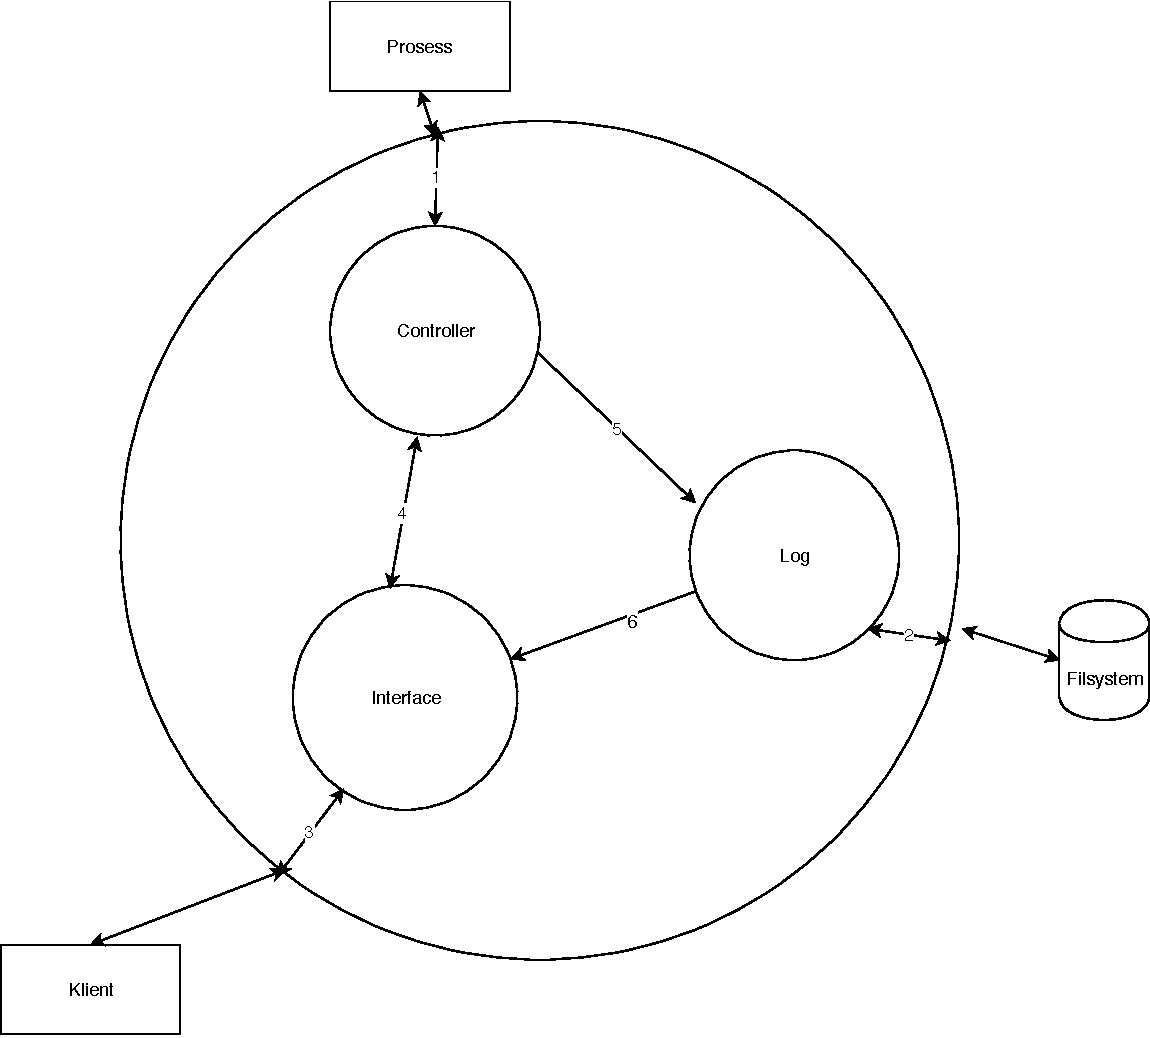
\includegraphics[width=\textwidth]{figures/system.pdf}
    \caption{Kontekstdiagram av hele systemet.}
    \label{fig:system}
\end{figure}

Totalt sett gir det ett design som ser ut som i figur \ref{fig:system}. Kommunikasjonen mellom modulene er følgende:
\begin{enumerate}
    \item Sensormålinger og pådrag.
    \item Lagring og lesing av logger og referanseserier.
    \item API-et beskrevet tidligere.
    \item Start av en prosess, lagring og lesing av referanseserier, og lesing av status på prosessen.
    \item Lagring av prosessverdier.
    \item Henting av logger.
\end{enumerate}


\begin{figure}
    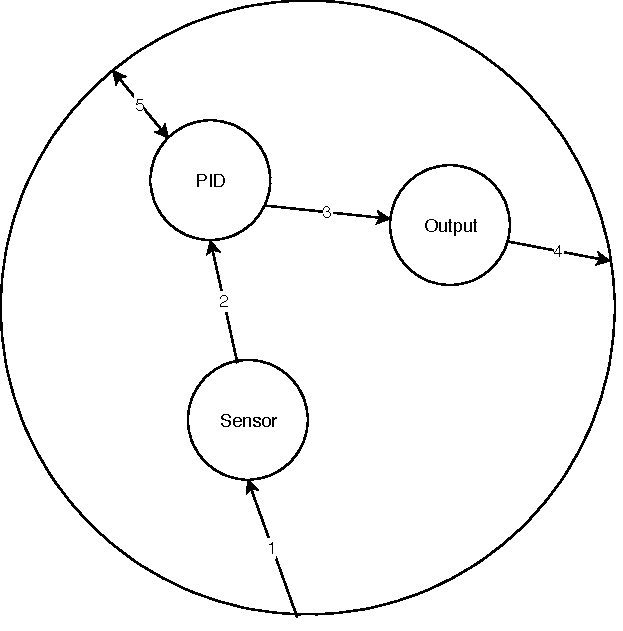
\includegraphics[width=\textwidth]{figures/controller.pdf}
    \caption{Kontekstdiagram for regulator-modulen.}
    \label{fig:regulator}
\end{figure}

Som nevnt er regulator-modulen den eneste som er litt komplisert designmessig. Sensor og Output modulene gir ett felles interface for ulike sensorer og pådragsorganer. PID modulen inneholder logikken til en PID-regulator. I tillegg har regulator-modulen en del logikk rundt oppstart og opprydning rundt prosessen. Hvordan modulen ser ut internt er vist i figur \ref{fig:regulator}, og kommunikasjonen knyttet til hver pil er listet opp nedenfor.
\begin{enumerate}
    \item Sensormålinger.
    \item Sensormålinger.
    \item Pådrag.
    \item Pådrag.
    \item Start av regulering, loggføring, lagring av referanseserier.
\end{enumerate}